\newpage
\section{Auswertung}

Um die aufgenommenen Daten zu analysieren werden die Python~\cite{python} Pakete NumPy~\cite{numpy} und SciPy~\cite{scipy} verwendet,
wobei Matplotlib~\cite{matplotlib} zum Erstellen von Grafiken und zudem Uncertainties~\cite{uncertainties} zur automatisierten
Fehlerfortpflanzung in linearer Ordnung dienen.

Nach einer Prüfung der Pulsform und Einrichtung der Diskriminatorschranken wird die Koinzidenzschaltung auf ihr zeitliches
Auflösungsvermögen geprüft. Anschließend muss den Kanälen des Vielkanalanalysators jeweils eine Zeit zugeordnet werden,
bevor mit der eigentlichen Langzeitmessung fortgefahren werden kann.



\subsection{Justageschritt}

Durch direktes Abgreifen der Signale beider Photomultiplier lässt sich am Oszilloskop der in Abbildung \ref{fig:pulse} gezeigte
Verlauf beobachten. Hier entsprechen die Kanäle 1 und 2 jeweils dem im Aufbau vorderen oder rechten sowie hinteren oder linken
PMT. Zunächst fällt auf, dass Peak 1 bei gleicher Skalierung eine signifikant geringere Amplitude als Peak 2
aufweist. Außerdem treten in Kanal 2 deutlich mehr Pulse auf, eine Beobachtung die auch am Diskriminatorausgang bestehen bleibt.
Auch durch Justieren des Schrankenwerts lässt sich das nicht ändern, wogegen die Einstellung von Kanal 1 auf die benötigten
$\qty{30}{\per\second}$ erfolgreich ist. Mithilfe der Koinzidenzschaltung sollte dieser Fehler demnach kompensiert werden.

\begin{figure}[H]
	\vspace{\baselineskip}
	\centering
	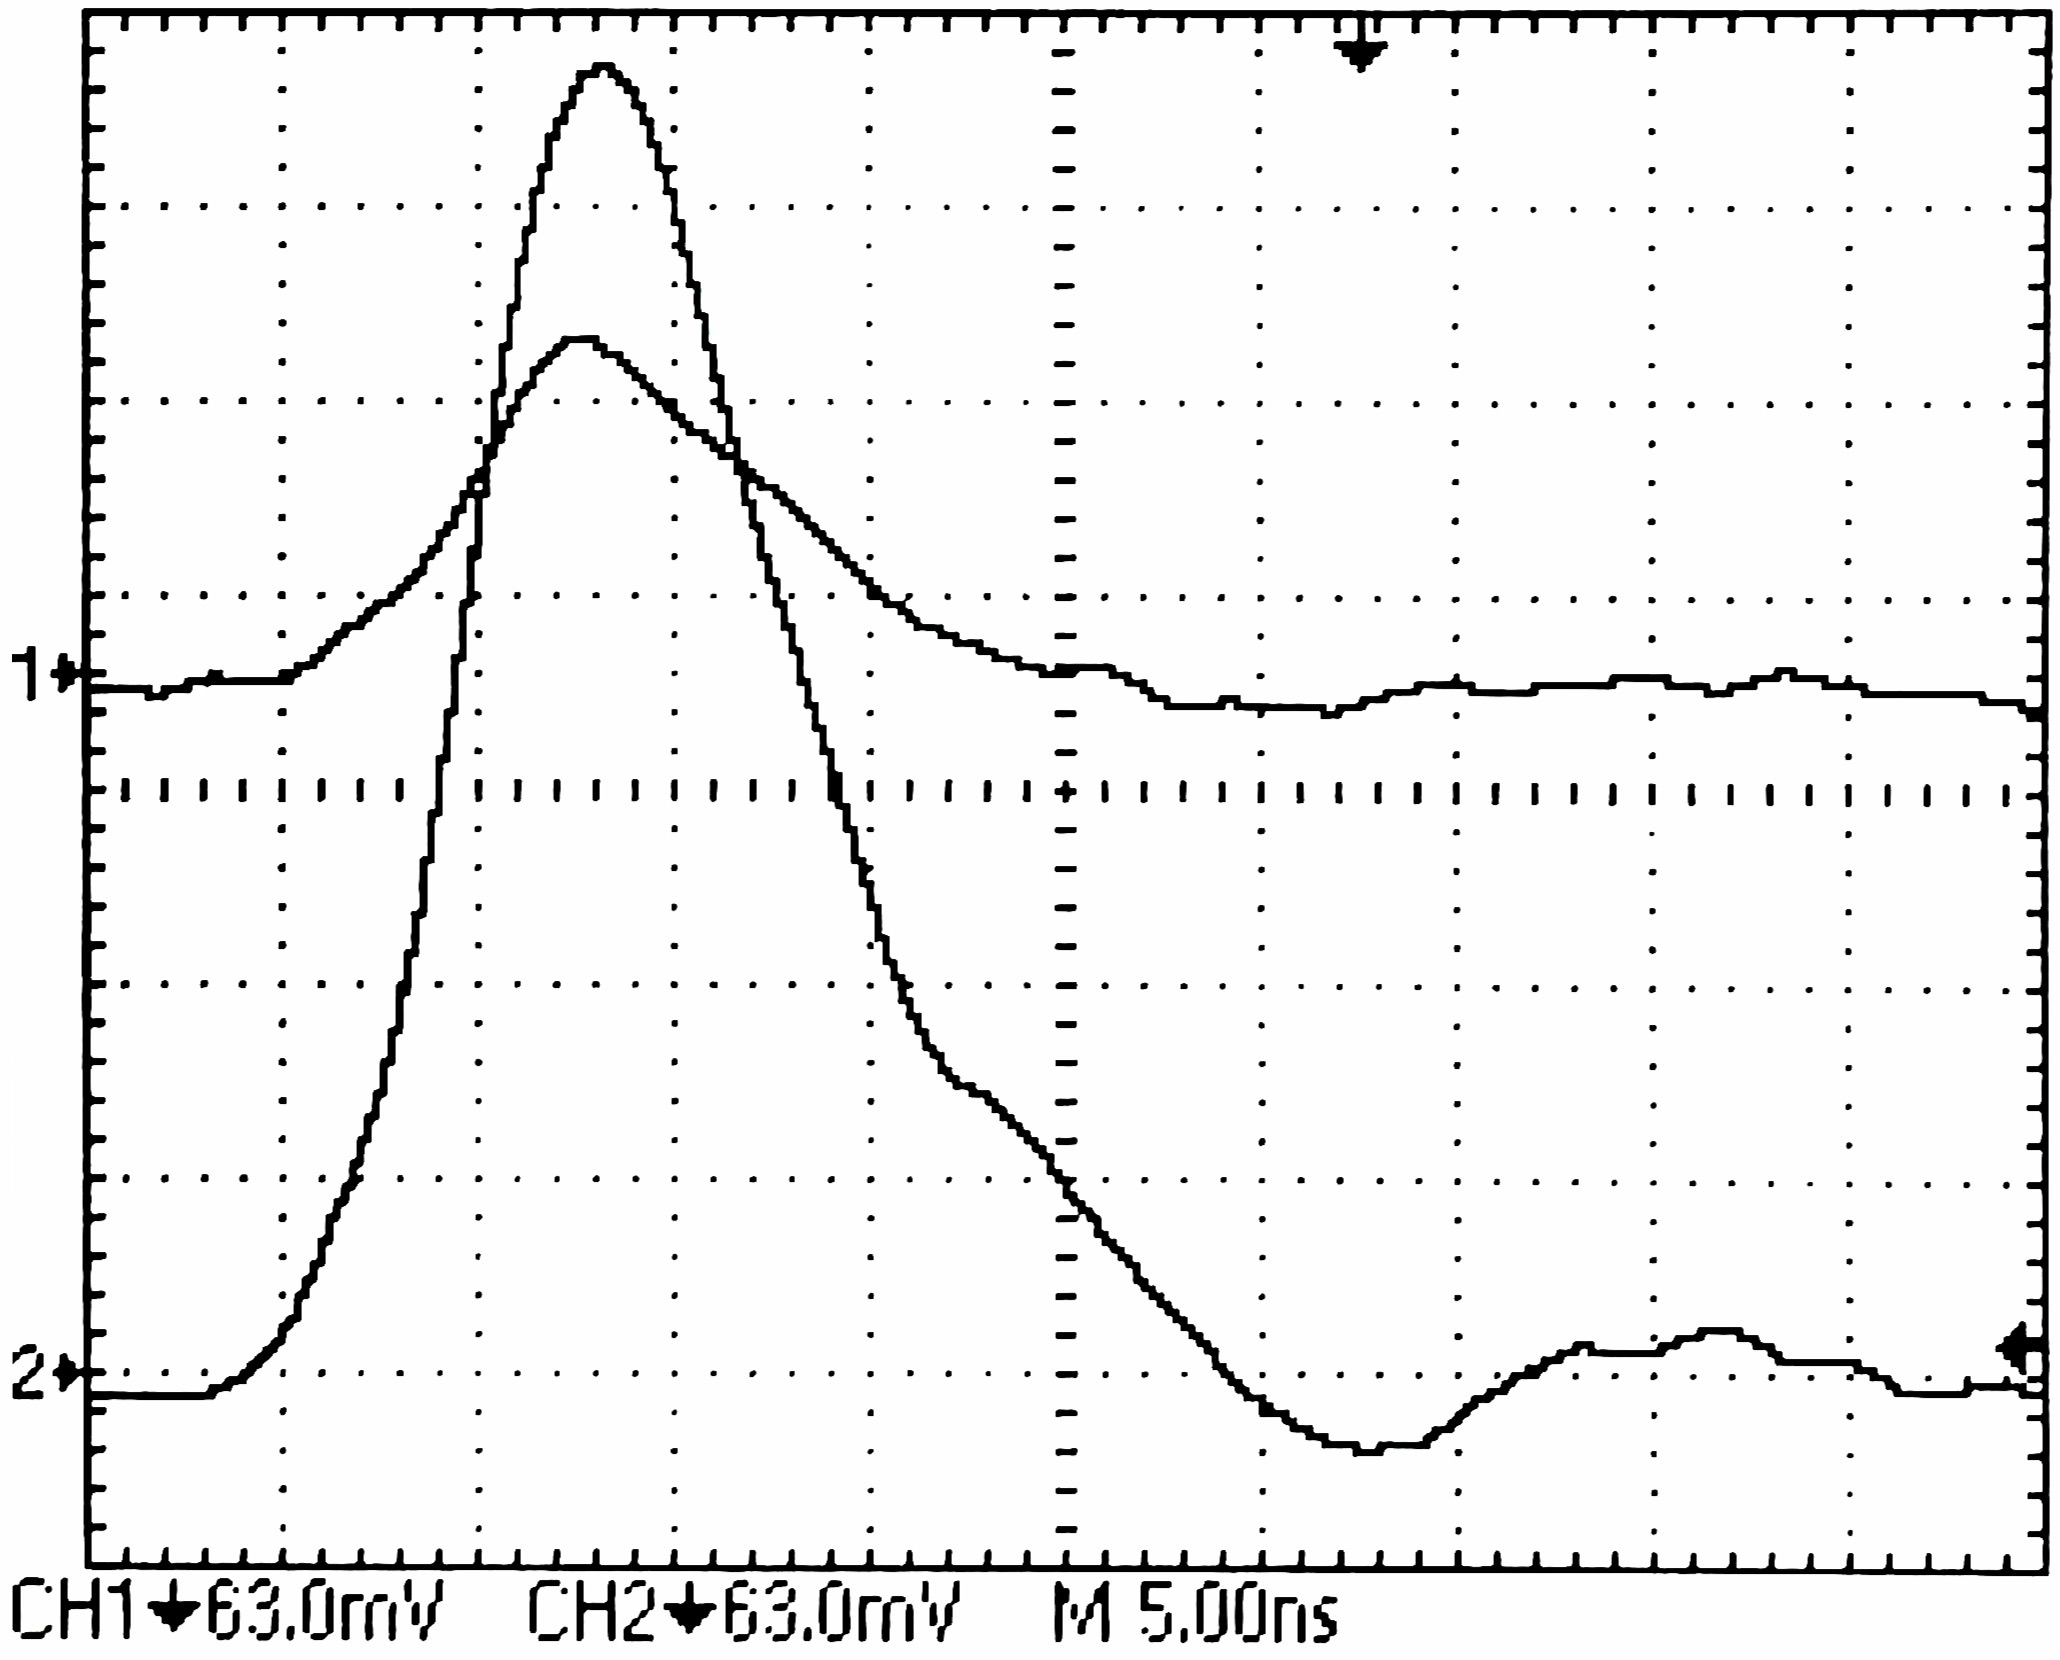
\includegraphics[width=0.6\textwidth]{content/messung/pulse.jpg}
	\caption{Am Oszilloskop aufgenommene Pulsformen aus den Photomultipliern.}
	\label{fig:pulse}
\end{figure}

Anhand Abbildung \ref{fig:pulse} kann zusätzlich der Vorteil eines Constant Fraction Discriminators veranschaulicht werden, indem
die eigentlich gleichzeitigen Verläufe als Beispiele für unterschiedlich hohe, zeitlich versetzte Pulse mit annäherend gleicher
Form am selben Diskriminator verwendet werden. Ein festgelegter Schwellenwert würde dann aufgrund der Skalierung zu einer
amplitudenabhängigen Verschiebung der Ausgangspulse führen und so die Messung verfälschen. Im gegebenen Fall wird stattdessen bei
einem bestimmten Bruchteil des Maximums ausgelöst, sodass dieser Fehler vermieden wird.

\begin{figure}[H]
	\vspace{\baselineskip}
	\begin{subfigure}{0.48\textwidth}
		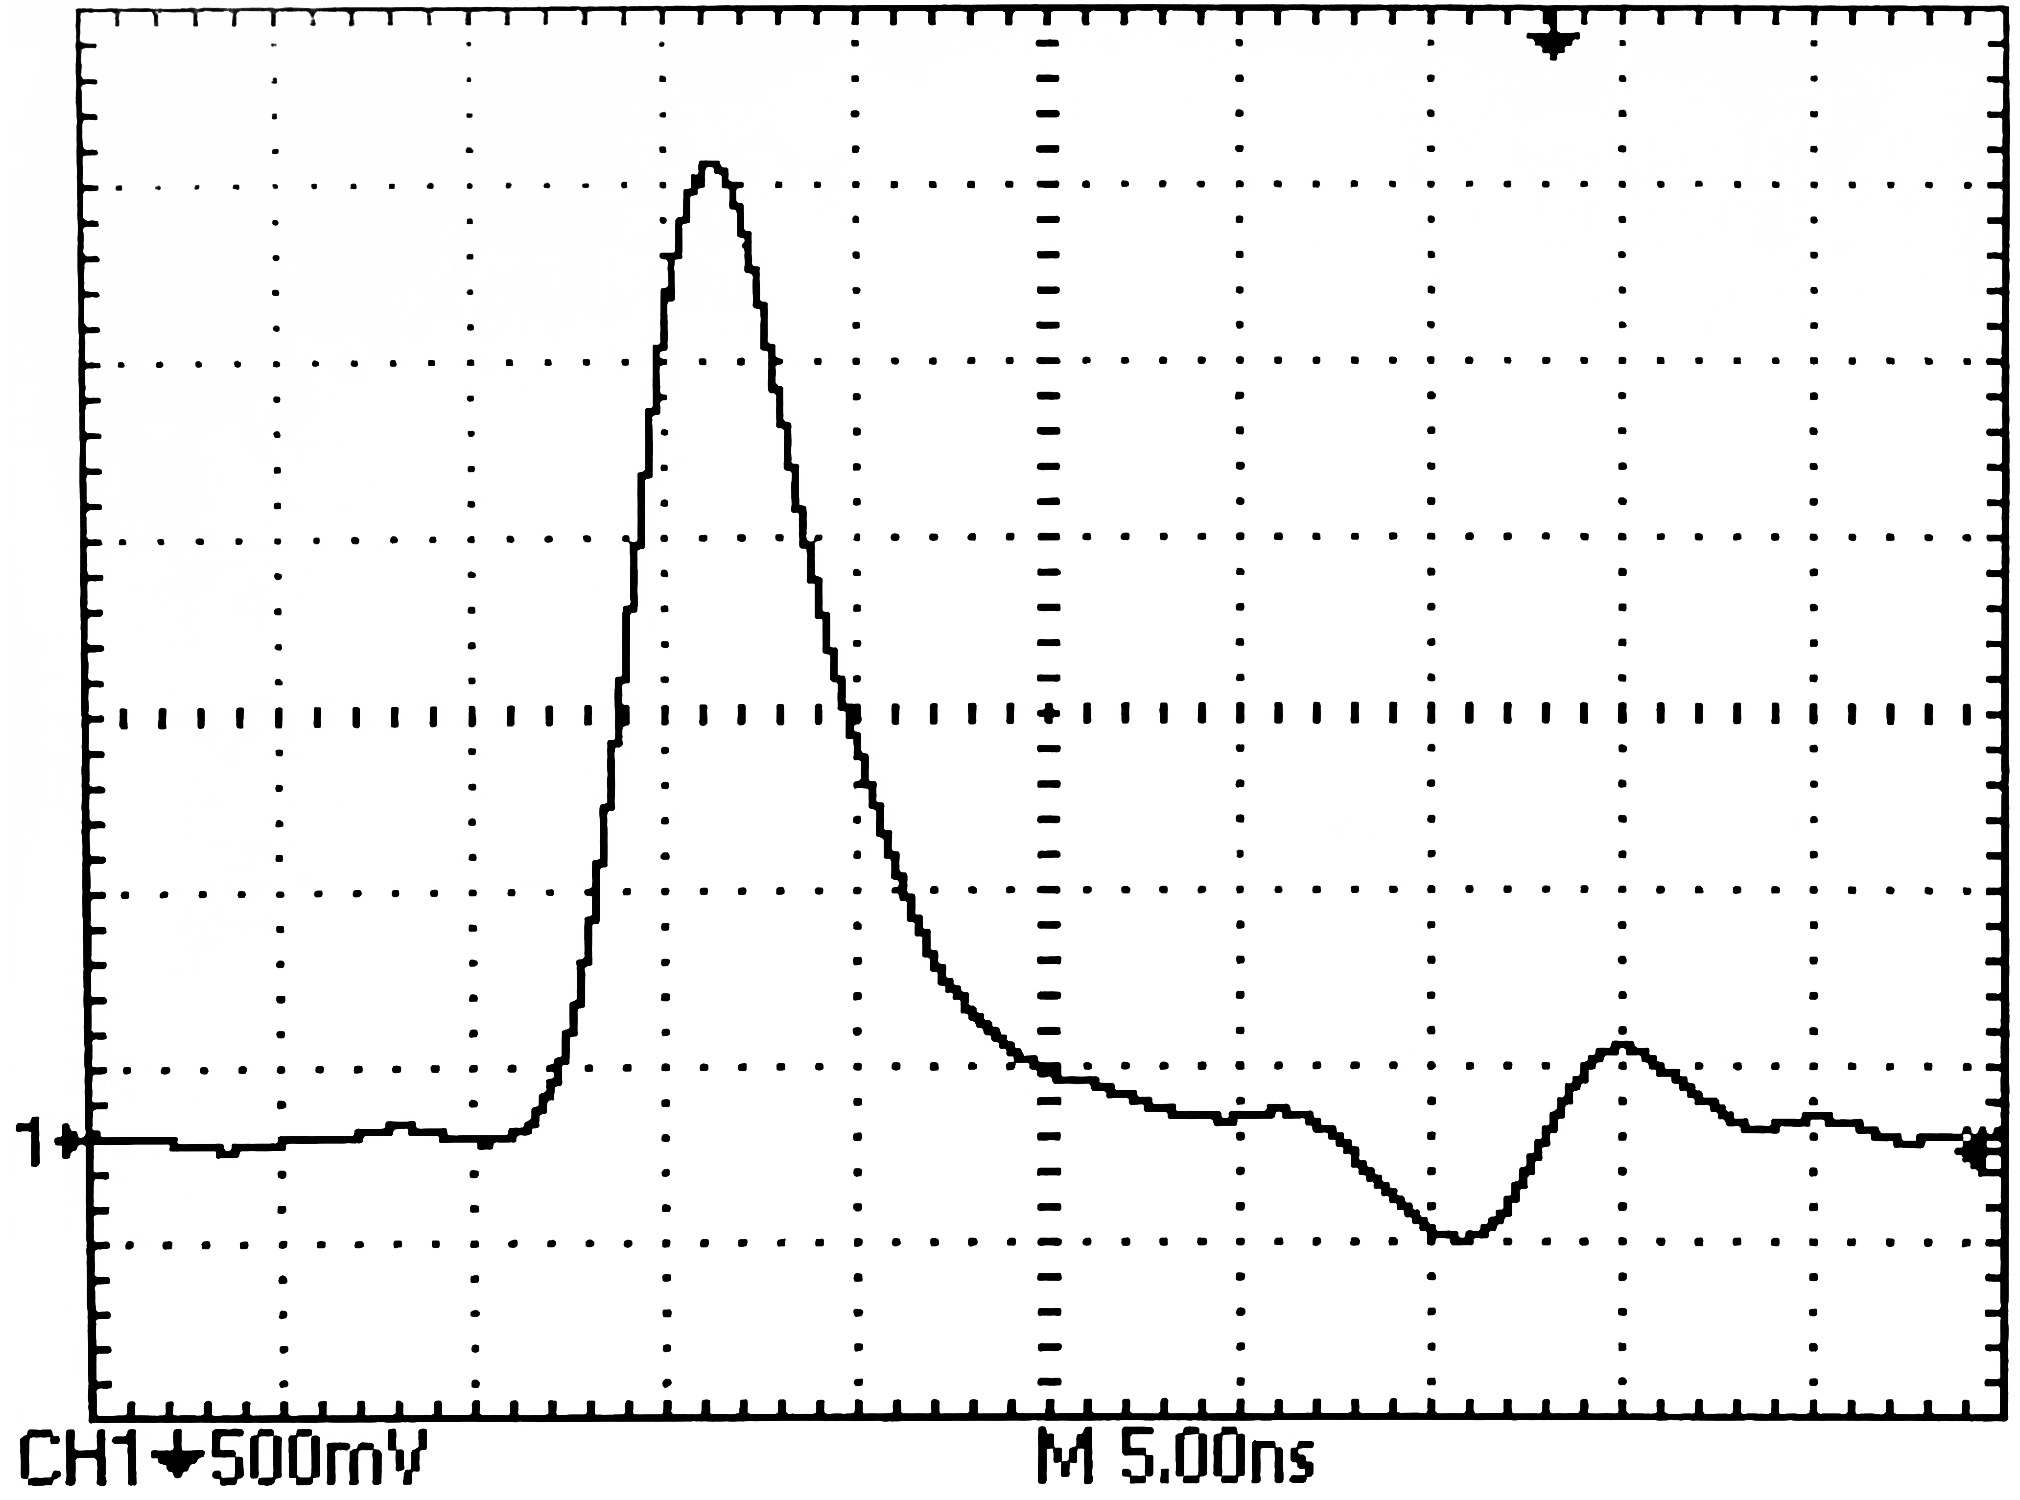
\includegraphics[width=\textwidth]{content/messung/unfiltered.jpg}
		\caption{Puls vor Diskriminator.}
	\end{subfigure}
	\hfill
	\begin{subfigure}{0.48\textwidth}
		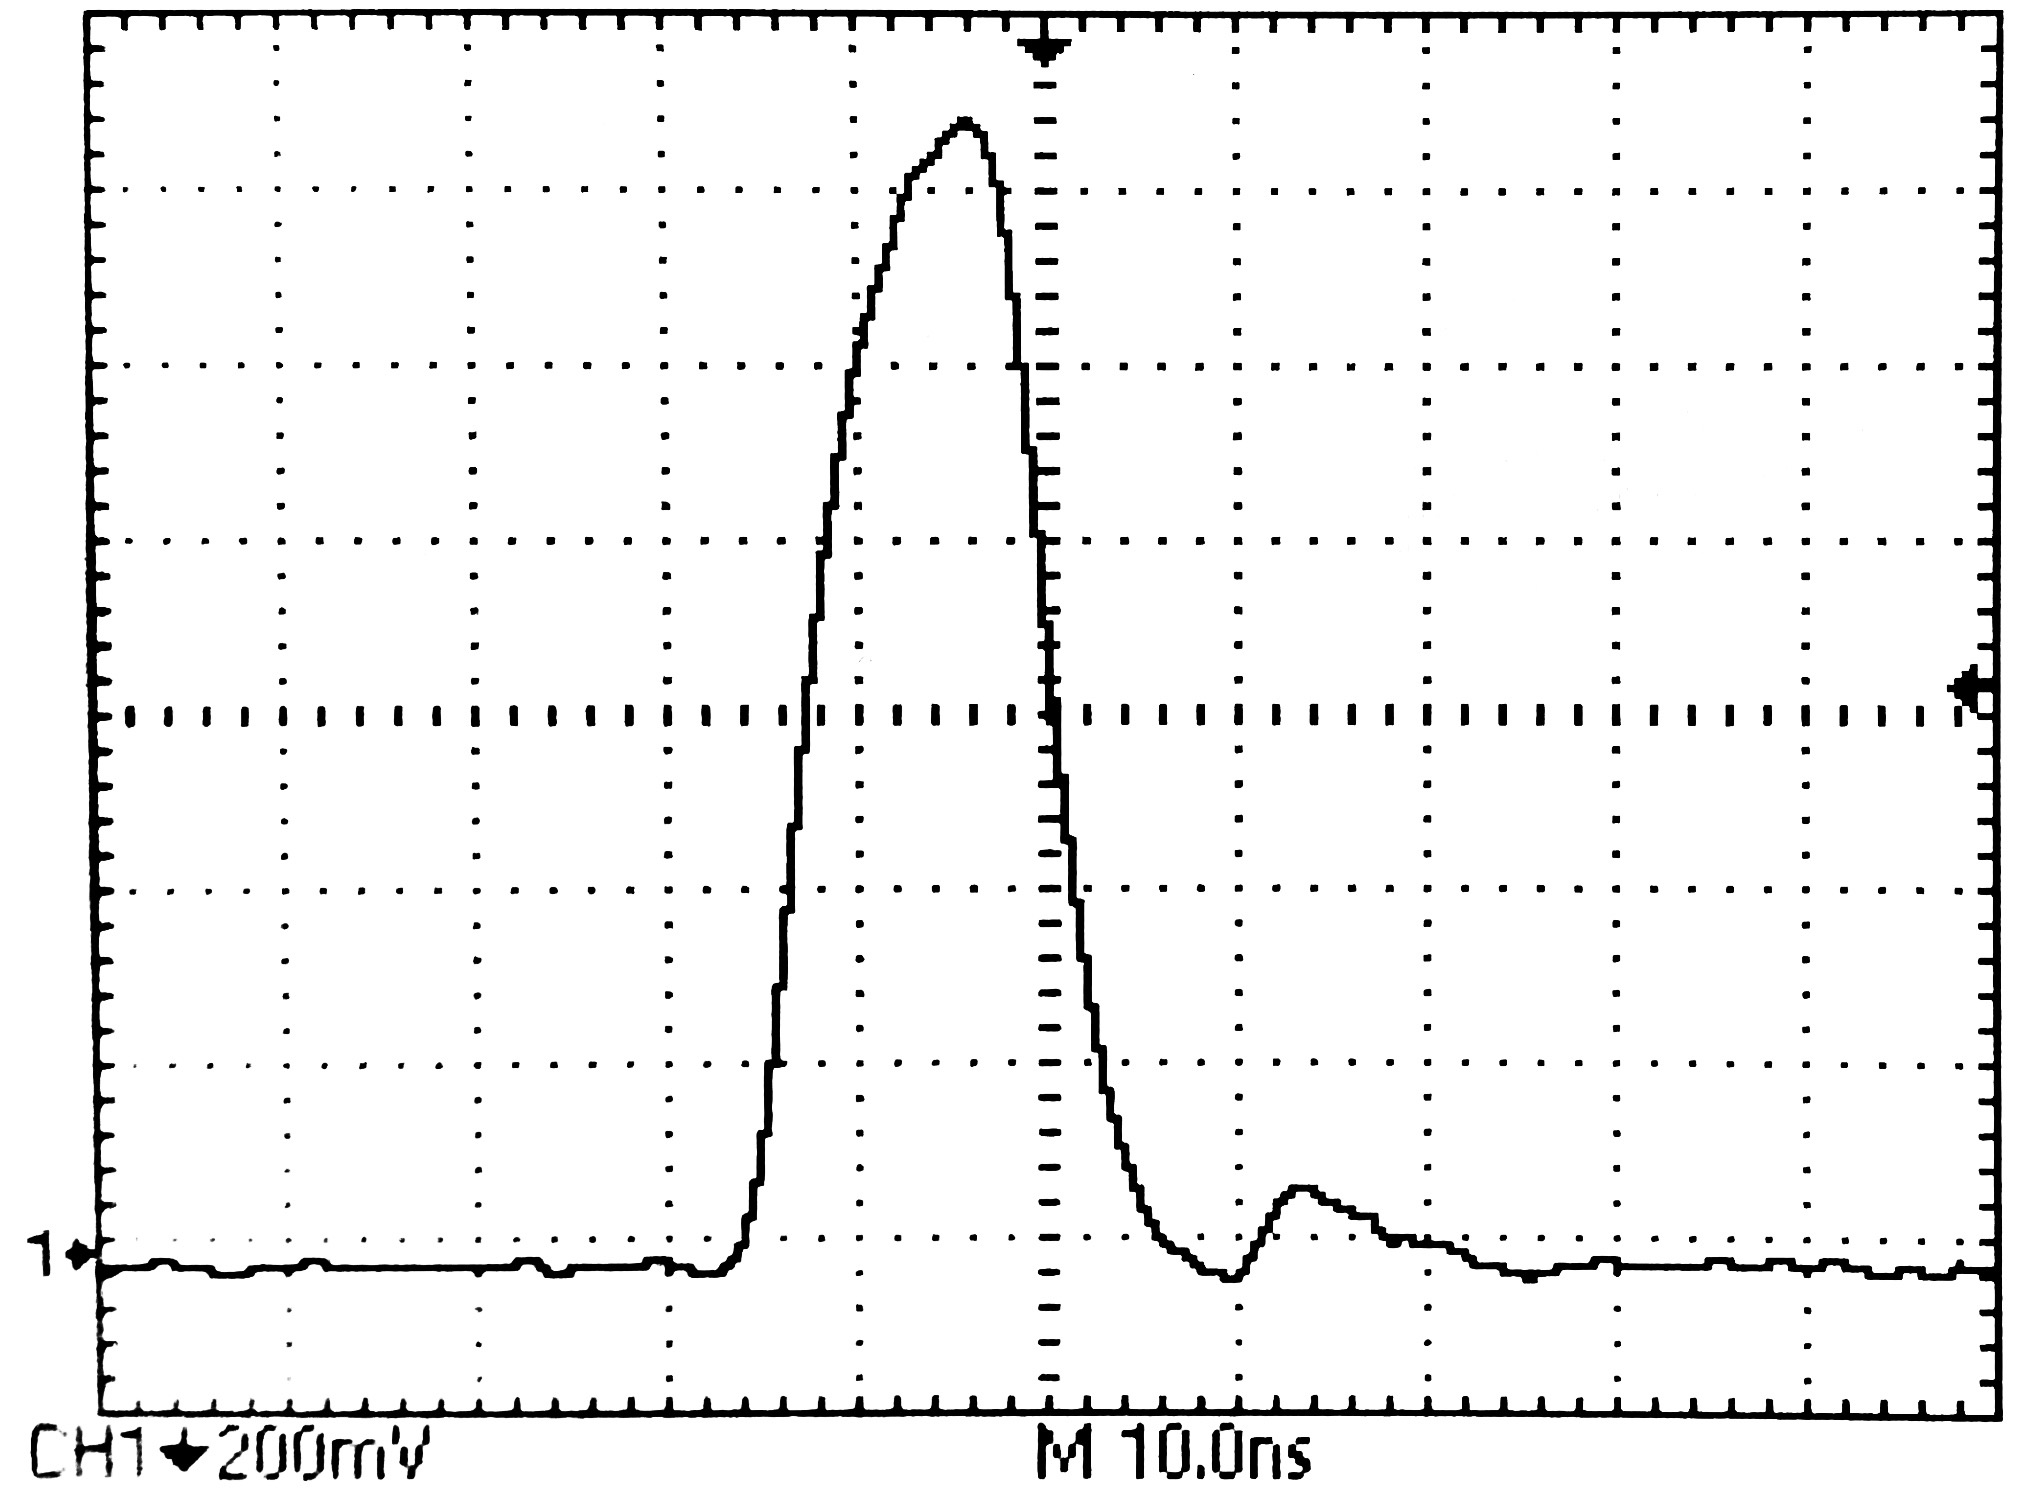
\includegraphics[width=\textwidth]{content/messung/filtered.jpg}
		\caption{Puls nach Diskriminator.}
	\end{subfigure}
	\caption{Vergleich der Pulsform vor und nach der Diskriminatorstufe.}
	\label{fig:filter}
\end{figure}

In Abbildung \ref{fig:filter} sind Signale ohne und mit zwischengeschaltetem Diskriminator dargestellt. Für das endgültige Signal
lässt sich signifikant weniger Rauschen beobachten. Ausßerdem kann am Diskriminatorausgang die Breite eingestellt werden. Damit
werden Pulse mit Maxima der Ordnung $\qty{1}{\volt}$ und Halbwertsbreiten von etwa $\qty{10}{\nano\second}$ in die
Koinzidenzschaltung gegeben, wobei die Zählrate aus dem ersten PMT etwa eine Größenordnung geringer als die des
zweiten ist.



\subsection{Verzögerungszeit}

Neben der Funktion zur Störunterdrückung durch Redundanz erlaubt der Aufbau mit zwei Photomultipliern auch eine eindimensional
räumliche Einstellung des verwendeten Volumens im organischen Szintillationsmedium, da die Verzögerung des Lichtblitzes im Bereich
der Auflösung der Koinzidenzschaltung liegt. Der Verlauf der in Tabelle \ref{tab:delay} gezeigten Messdaten wird in Abbildung
\ref{fig:delay} als Trapez mit Null als Asymptote genähert.

Per Ausgleichsrechnung ergibt sich
\begin{equation*}
	a = \qty{1.7+-0.1}{\per\nano\second}
\end{equation*}
für die Steigung der positiven Flanke.

Es folgen außerdem die Knickstellen
\begin{align*}
	b &= \qty{-11.6+-0.3}{\nano\second} \: , & c &= \qty{-0.1+-0.4}{\nano\second} \: , \\
	d &= \qty{8.1+-0.9}{\nano\second} \: , & e &= \qty{17.3+-0.3}{\nano\second} \: .
\end{align*}

\begin{figure}[H]
	\centering
	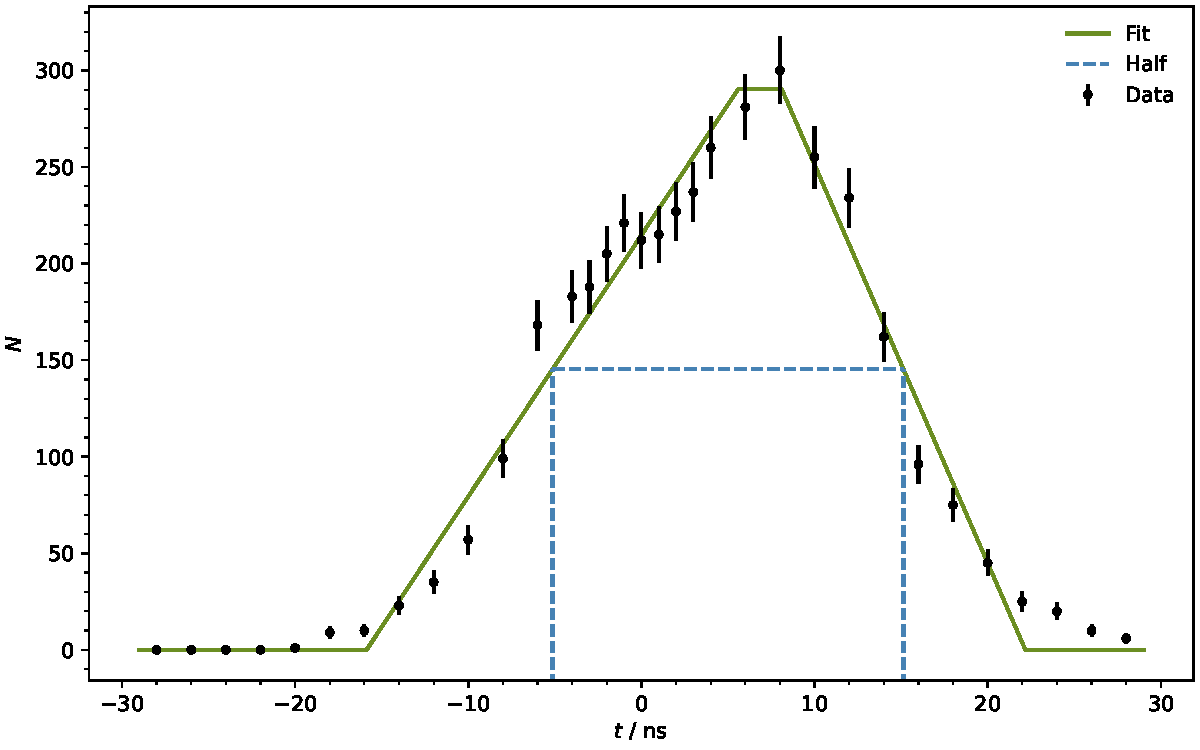
\includegraphics[width=\textwidth]{build/delay.pdf}
	\caption{Gemessene Zählraten gegen die eingestellte Verzögerung.}
	\label{fig:delay}
\end{figure}

Daraus lassen sich einige relevante Größen berechnen. Die maximale Zählrate, für die ein Zielwert von $\qty{20}{\per\second}$
angegeben ist, lautet
\begin{equation*}
	N_\text{Plateau} = \num{20+-1}
\end{equation*}
im Bereich des Plateaus, welches eine Breite
\begin{equation*}
	T_\text{Plateau} = \qty{5.3+-0.5}{\nano\second}
\end{equation*}
aufweist. Bei den Zeiten
\begin{align*}
	t_\text{links} = \qty{-5.9+-0.2}{\nano\second} \: , && t_\text{rechts} = \qty{11.2+-0.2}{\nano\second}
\end{align*}
ist die Hälfte dieses Maximums erreicht.

Damit folgt die Halbwertsbreite
\begin{equation*}
	T_\text{Hälfte} = t_\text{rechts} - t_\text{links} = \qty{20.3+-0.8}{\nano\second}
\end{equation*}
und letztendlich eine mittlere Anstiegszeit
\begin{equation*}
	T_\text{Anstieg} = T_\text{Hälfte} - T_\text{Plateau} = \qty{11.8+-0.3}{\nano\second} \: .
\end{equation*}
Um für weitere Messungen eine maximale Zählrate zu erzielen, wird die Verzögerung
\begin{equation*}
	t_\text{optimal} = \qty{6.8+-0.7}{\nano\second}
\end{equation*}
entsprechend der Mitte des Plateaus eingestellt.



\subsection{Kanalkalibration}

Ausgehend von der Umwandlung der gemessenen Zeitdifferenz von Eintreten und Zerfall zur Eingangsamplitude am
Vielkanalanalysator wird ein linearer Zusammenhang zwischen Kanalnummer $K$ und der Zeit $t$ angesetzt. Sollte
die Zuordnung zu zwei benachbarten Kanälen erfolgen, wird der Mittelwert der Indizes verwendet.

\begin{figure}[H]
	\vspace{\baselineskip}
	\centering
	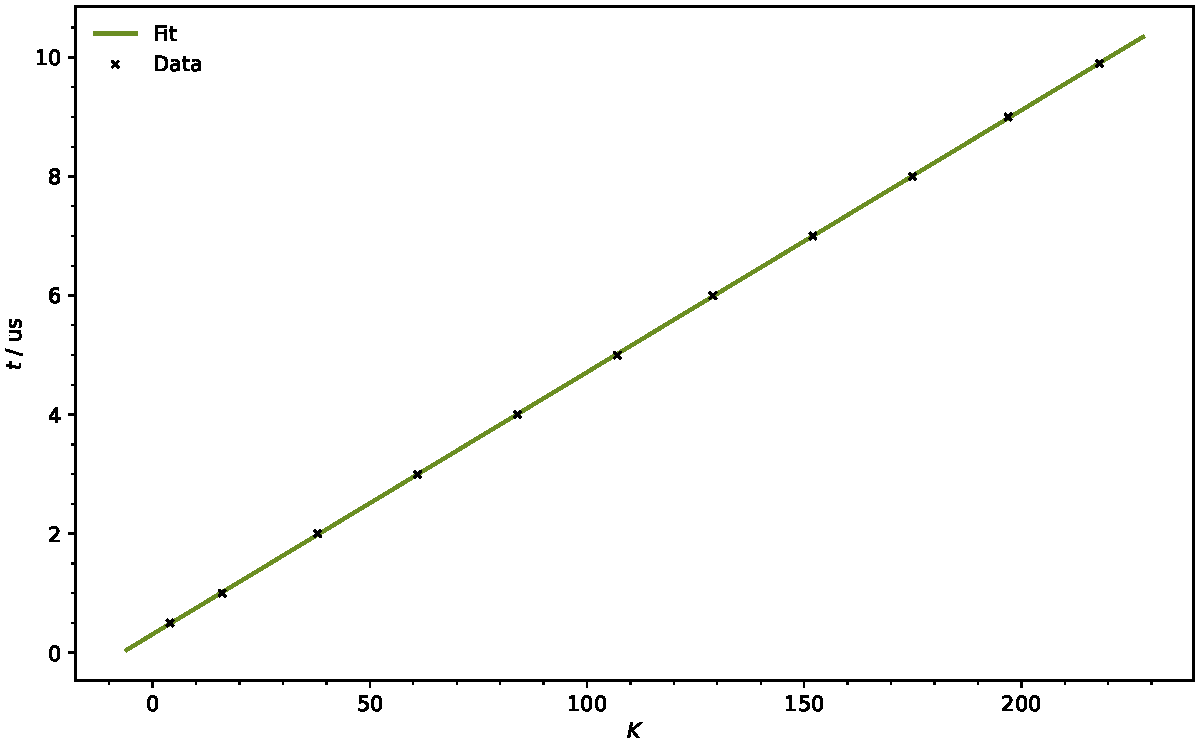
\includegraphics[width=\textwidth]{build/calibration.pdf}
	\caption{Beobachteter Zusammenhang zwischen Kanalnummer und Zeitskala.}
	\label{fig:calibration}
\end{figure}

Aus der entsprechenden Formel für die Umrechnung von Kanal zu Zeitskala
\begin{equation*}
	t(K) = AK + B
\end{equation*}
bestimmen sich die in Abbildung \ref{fig:calibration} verwendeten Parameter
\begin{align*}
	A = \qty{0.02167+-0.00001}{\micro\second} \: , && B = \qty{0.313+-0.008}{\micro\second} \: .
\end{align*}
Diese Werte ergeben sich, indem an die Daten aus Tabelle \ref{tab:calibration} angepasst wird. Daran lässt sich ebenfalls
eine global homogene Effizienz feststellen, da im Messintervall ähnliche Zählraten unabhängig der Kanalnummer auftreten.
Dies lässt sich auch an der relativ geringen Streuung des Mittelwerts $\qty{1013+-10}{\second}$ verifizieren, welcher in etwa mit
der am Doppelpulsgenerator gegebenen Frequenz von $\qty{1000}{\second}$ übereinstimmt.



\subsection{Langzeitmessung}

Für die Messung der Zählrate $N$ gegen die Zeitdifferenz $t$ aus Tabelle \ref{tab:lifetime} lässt sich
\begin{equation*}
	N(t) = m + ne^{-\lambda t}
\end{equation*}
als exponentieller Zusammenhang mit Normierung $n$ ansetzen, der um $m$ als Hintergrund verschoben ist. Aufgrund der
beobachteten Streuung werden ausschließlich die Kanäle mit Indizes $\num{4}$ bis $\num{226}$
verwendet und in Abbildung \ref{fig:lifetime} aufgetragen.

\begin{figure}[H]
	\centering
	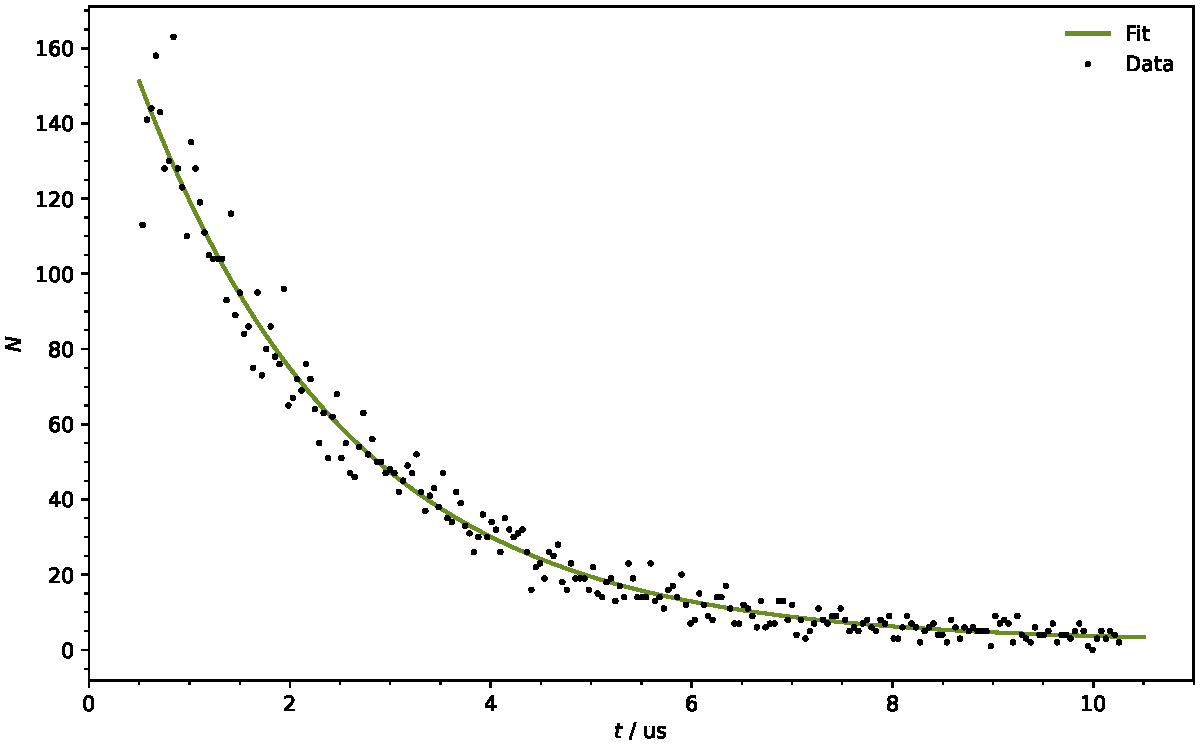
\includegraphics[width=\textwidth]{build/lifetime.pdf}
	\caption{Daten aus der Langzeitmessung mit exponentieller Fitfunktion.}
	\label{fig:lifetime}
	\vspace{-\baselineskip}
\end{figure}

Die Werte der genannten Parameter lauten
\begin{align*}
	m = \num{2.03(0.01)} \: , && n = \num{186.1+-2.7} \: .
\end{align*}
Zusätzlich ergibt sich
\begin{equation*}
	\lambda = \qty{0.44+-0.02}{\per\micro\second}
\end{equation*}
als Zerfallskonstante und schließlich
\begin{equation*}
	\tau = \qty{1.03+-0.03}{\micro\second}
\end{equation*}
für die Lebensdauer kosmischer Myonen, wobei $\qty{2.197}{\micro\second}$ den Literaturwert angibt \cite{Tishchenko_2013}.



\subsection{Hintergrundrate}

Anhand der charakterisierenden Eigenschaften der Messreihe
\begin{align*}
	T_\text{such} &= \qty{10}{\micro\second} \: , & T_\text{mess} &= \qty{158234}{\second} \: , \\
	N_\text{start} &= \num{4509112} \: , & N_\text{stopp} &= \num{17526}
\end{align*}
lässt sich ein Erwartungswert
\begin{equation*}
	\langle N \rangle = N_\text{start} \frac{T_\text{such}}{T_\text{mess}} = \num{0.000285}
\end{equation*}
für die Zählrate innerhalb des Suchzeitintervalls aufstellen. Unter der Annahme einer für Zählexperimente gültigen
Poissonverteilung
\begin{equation*}
	P_k = \pfrac{\langle N \rangle ^k}{k!} e^{-\langle N \rangle}
\end{equation*}
folgt für die Wahrscheinlichkeit, dass genau ein weiteres Myon einfällt,
\begin{equation*}
	P_1 = \qty{0.0191}{\percent} \: .
\end{equation*}
Somit lässt sich die Anzahl zusätzlicher Pulse zu
\begin{equation*}
	O_1 = P_1 N_\text{start} = \num{562}
\end{equation*}
abschätzen, welche sich homogen über $\num{512}$ Kanäle verteilen. Pro Kanal gilt demnach
\begin{equation*}
	M = \num{2.5}
\end{equation*}
als Hintergrundrate, die mit dem Wert $m = \num{2.03(0.01)}$ aus dem vorherigen Vorgehen verglichen werden kann.
